\documentclass[11pt]{article}

% ---------- preamble (arXiv-style preprint) ----------
\PassOptionsToPackage{hyphens}{url}
\usepackage[margin=1in]{geometry}
\usepackage[T1]{fontenc}
\usepackage[utf8]{inputenc}
\usepackage{mathptmx}
\usepackage{microtype}
\usepackage{amsmath,amssymb}
\usepackage{booktabs}
\usepackage{graphicx}
\usepackage{xcolor}
\usepackage{caption}
\usepackage{subcaption}
\usepackage{enumitem}
\usepackage{algorithm}
\usepackage{algpseudocode}
\usepackage{tikz}
\usetikzlibrary{arrows.meta,positioning,shapes.misc}
\usepackage[numbers,sort&compress]{natbib}
\usepackage[colorlinks=true,linkcolor=blue!55!black,citecolor=blue!55!black,urlcolor=blue!55!black]{hyperref}
\usepackage{xurl}
\captionsetup{font=small,labelfont=bf,skip=4pt}
\setlist{nosep,leftmargin=*}
\graphicspath{{figures/}}
\newcommand{\nvarc}{NVARC}
\newcommand{\mega}{ARC-Mega}
\newcommand{\todo}[1]{\textcolor{red}{[#1]}}

\title{\textbf{Let the Solver Choose Its Data:}\\[2pt]
\large Likelihood-Band Selection of Synthetic ARC-AGI-2 Tasks, and Why Held-Out Loss Is the Wrong Signal}

\author{Harthik Mallichetty\\
Independent researcher, Dallas, TX\\
\texttt{hrmallichetty@gmail.com}\quad Kaggle: \texttt{harthikrm}}
\date{ARC Prize 2026 Paper Track \quad $\cdot$ \quad November 2026}

\begin{document}
\maketitle

\begin{abstract}
Large synthetic task pools now exist for the Abstraction and Reasoning Corpus, but most of their contents are either already solved by a strong solver or unlearnable by it. We propose \emph{solver-in-the-loop} curation: score every candidate task with the target solver's own zero-shot teacher-forced likelihood of the answer (one forward pass, no decoding, no labels beyond the task itself), and keep only the tasks whose per-token negative log-likelihood (NLL) falls inside the band spanned by the target benchmark's 25th--95th percentiles and that the solver does not already solve greedily. Applied to \mega{}~\citep{arcmega2025}, the method scores 114{,}067 tasks in $\approx$8.4 hours on Kaggle's 4$\times$L4 machine and retains 42\%. Continue-training the 2025-winning \nvarc{} model~\citep{nvarc2025} on only 6{,}000 selected tasks (0.008\% of the pool's ARC tasks, 2 GPU-hours on one H200) raised its hidden-test score on the ARC Prize 2026 leaderboard from a mean of 28.5 (three draws of the stock checkpoint) to 31.2 (two draws), with the unchanged test-time-training pipeline. Scaling the same recipe to 47{,}435 tasks lowered the held-out loss on selected tasks by 39\% but \emph{did not} improve the hidden score (29.6, one draw), while a forgetting monitor on the public evaluation set turned upward. We argue that the band works because it targets the solver's learning frontier, that in-distribution held-out loss is the wrong model-selection signal once the solver adapts per task at test time, and that a rise in the forgetting monitor is the earlier and cheaper warning. All code is released; the method needs only a solver that assigns likelihoods and is agnostic to how the pool was generated.
\end{abstract}

% =====================================================================
\section{Introduction}
ARC-AGI-2~\citep{chollet2025arcagi2} tests whether a system can infer a novel grid transformation from a few demonstrations. The 2025 Kaggle winner, \nvarc{}~\citep{nvarc2025}, is a transductive pipeline: a Qwen3-4B model~\citep{yang2025qwen3} fine-tuned on $\sim$100k LLM-generated puzzles, adapted to each test task with LoRA test-time training (TTT)~\citep{akyurek2024ttt}, decoded with depth-first search, and re-scored under augmentations~\citep{franzen2024architects,franzen2025architects}. Its public code and checkpoint became the starting point for a large fraction of the 2026 field.

In September 2026, MindsAI/Tufa Labs released \mega{}, a 134\,GB pool of roughly 97 million training rows, about 74 million of them ARC tasks~\citep{arcmega2025}. The pool is far larger than any single team can train on under a competition budget, and it is heterogeneous: our probe (\S\ref{sec:mega}) finds that 14.5\% of its profile-matched tasks are already solved greedily by \nvarc{} without any adaptation and that a further 10\% carry answer likelihoods below the benchmark's own 95th-percentile tail. The practical question for a resource-limited competitor is therefore not \emph{how to generate more data} but \emph{which of the abundant data to spend compute on}.

This paper answers that question with a method that needs nothing beyond the solver itself (Figure~\ref{fig:pipeline}). We compute, for each candidate task, the per-token NLL that the frozen solver assigns to the correct test output given the demonstrations, and we keep the task if (i) the solver does not already reproduce the output under greedy decoding and (ii) its NLL lies within the 25th--95th percentile band of the solver's NLL on the public ARC-AGI-2 evaluation set. Everything the solver already solves is kept as replay~\citep{rolnick2019replay}. The selected tasks are used for a short LoRA continuation of the solver's base checkpoint; the rest of the \nvarc{} pipeline is untouched.

\paragraph{Contributions.}
\begin{enumerate}
\item A label-free, one-forward-pass data-curation rule that matches a synthetic pool to a target benchmark \emph{through the solver's eyes}, together with a characterisation of \mega{} under it (\S\ref{sec:method}--\S\ref{sec:mega}).
\item Hidden-leaderboard evidence that 6k selected tasks improve \nvarc{} by $+2.7$ points on ARC Prize 2026 (\S\ref{sec:results}); the linked Kaggle submission is this model.
\item A negative scaling result: $8\times$ more selected data lowers the in-distribution held-out loss by 39\% yet does not improve the hidden score. We explain why held-out loss on the selected pool is the wrong signal once the solver adapts per task, and show that a forgetting monitor on the target benchmark flags the problem earlier (\S\ref{sec:analysis}).
\item A record of three further levers we measured and rejected under the same budget---answer re-ranking, CPU program search, and test-time program induction with 30B-class open models---so that others do not repeat them (\S\ref{sec:negative}).
\end{enumerate}

\begin{figure}[t]
\centering
\resizebox{\textwidth}{!}{%
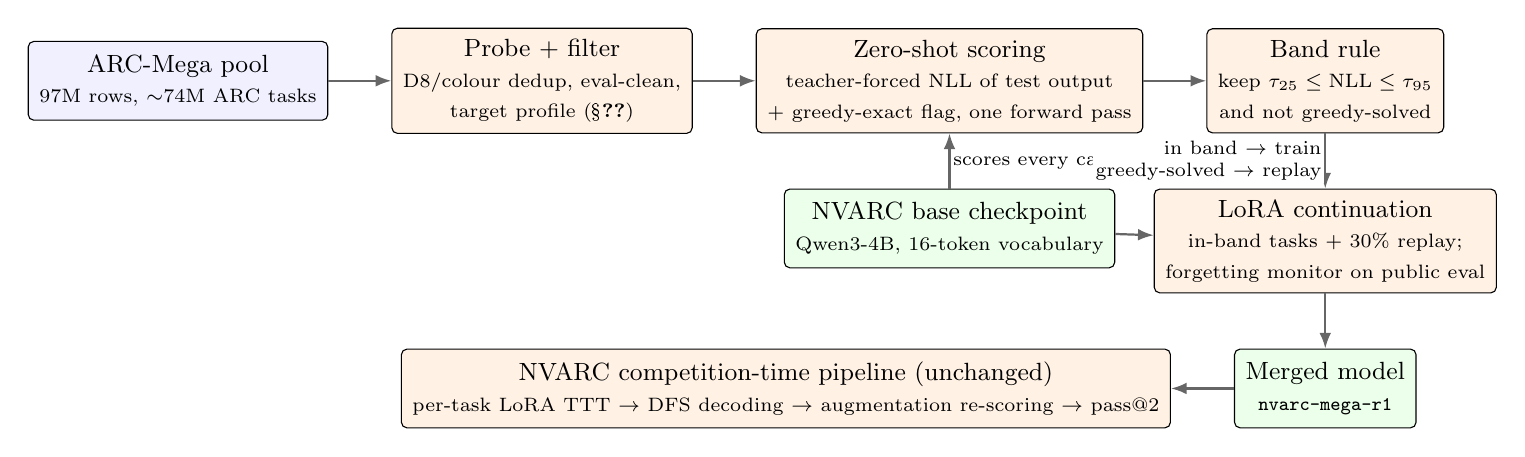
\begin{tikzpicture}[
  box/.style={draw,rounded corners=2pt,align=center,font=\small,minimum height=10mm,inner sep=4pt,fill=white},
  data/.style={box,fill=blue!6},
  proc/.style={box,fill=orange!10},
  model/.style={box,fill=green!8},
  arr/.style={-{Latex[length=2mm]},thick,draw=black!60},
  lab/.style={font=\scriptsize,fill=white,inner sep=1pt},
  node distance=7mm and 8mm]
\node[data] (mega) {\mega{} pool\\ \scriptsize 97M rows, $\sim$74M ARC tasks};
\node[proc,right=of mega] (probe) {Probe + filter\\ \scriptsize D8/colour dedup, eval-clean,\\ \scriptsize target profile (\S\ref{sec:mega})};
\node[proc,right=of probe] (score) {Zero-shot scoring\\ \scriptsize teacher-forced NLL of test output\\ \scriptsize + greedy-exact flag, one forward pass};
\node[proc,right=of score] (band) {Band rule\\ \scriptsize keep $\tau_{25}\le \mathrm{NLL}\le\tau_{95}$\\ \scriptsize and not greedy-solved};
\node[model,below=of score] (base) {\nvarc{} base checkpoint\\ \scriptsize Qwen3-4B, 16-token vocabulary};
\node[proc,below=of band] (train) {LoRA continuation\\ \scriptsize in-band tasks + 30\% replay;\\ \scriptsize forgetting monitor on public eval};
\node[model,below=of train] (merged) {Merged model\\ \scriptsize \texttt{nvarc-mega-r1}};
\node[proc,left=of merged] (ttt) {\nvarc{} competition-time pipeline (unchanged)\\ \scriptsize per-task LoRA TTT $\to$ DFS decoding $\to$ augmentation re-scoring $\to$ pass@2};
\draw[arr] (mega)--(probe); \draw[arr] (probe)--(score); \draw[arr] (score)--(band);
\draw[arr] (base)--node[lab,right]{scores every candidate}(score);
\draw[arr] (base)--(train);
\draw[arr] (band)--node[lab,left,align=right]{in band $\to$ train\\ greedy-solved $\to$ replay}(train);
\draw[arr] (train)--(merged);
\draw[arr] (merged)--(ttt);
\end{tikzpicture}}
\caption{Solver-in-the-loop curation. The frozen solver scores every candidate once; the band rule keeps tasks at the solver's learning frontier; greedy-solved tasks become replay. Only the base checkpoint changes; the competition-time pipeline is the public \nvarc{} code.}
\label{fig:pipeline}
\end{figure}

% =====================================================================
\section{Background and related work}
\paragraph{ARC and transductive solvers.}
ARC~\citep{chollet2019measure} tasks present 2--7 demonstration pairs of coloured grids and one or two test inputs; a prediction is correct only if every cell matches, with two attempts per test input (pass@2). The dominant Kaggle approach since 2024 fine-tunes a small language model on grid-to-grid examples and adapts it per task at test time~\citep{franzen2024architects,akyurek2024ttt,franzen2025architects}. \nvarc{}~\citep{nvarc2025} added a four-stage synthetic data pipeline (puzzle descriptions from H-ARC and BARC, LLM-mixed descriptions, generated input programs, consistency-filtered output programs) and full fine-tuning on 3.2M augmented samples. Its authors report that validation loss on augmented public-evaluation puzzles correlated with the public leaderboard; our results qualify that observation (\S\ref{sec:analysis}). Inductive (program-synthesis) solvers~\citep{li2024induction,hodel2024rearc,wind2020icecuber} and recursive tiny models~\citep{jolicoeur2025trm} are complementary; we measured both under our budget (\S\ref{sec:negative}).

\paragraph{Synthetic ARC data.}
Re-ARC~\citep{hodel2024rearc} provides generators for the 400 ARC-AGI-1 training tasks; BARC~\citep{li2024induction} and \nvarc{} generate new tasks with LLM-written programs; \mega{}~\citep{arcmega2025} aggregates MindsAI training data at a scale (97M training rows, $\sim$74M ARC tasks) two orders of magnitude beyond prior releases. Prior work asks how to \emph{generate} such pools; we ask how to \emph{select} from one when training compute is the binding constraint.

\paragraph{Loss-based data selection.}
Selecting examples by a model's own loss has a long history: curriculum learning~\citep{bengio2009curriculum}, RHO-LOSS, which prioritises points that are ``learnable, worth learning, and not yet learnt''~\citep{mindermann2022rholoss}, dataset cartography~\citep{swayamdipta2020cartography}, and perplexity-based pruning for LLM pre-training~\citep{marion2023lessismore,ankner2024perplexed}. \citet{sorscher2022beyond} show that in the data-abundant regime one should keep \emph{hard} examples but that the hardest fraction is harmful. Gradient-based selection~\citep{xia2024less} targets a downstream distribution at a higher cost. Our rule is a cheap instance of this family specialised to the ARC setting: the \emph{target solver} is the reference model, the difficulty band is anchored to the \emph{target benchmark's} percentiles rather than to fixed thresholds, and ``already learnt'' is operationalised by greedy exact-match, which is the actual success criterion for ARC.

% =====================================================================
\section{Method}
\label{sec:method}

\subsection{Zero-shot likelihood scoring}
Let $S_\theta$ be the frozen solver and let a task $t$ consist of demonstrations $D=\{(x_i,y_i)\}$ and a test pair $(x^\ast,y^\ast)$. We serialise $(D,x^\ast)$ in \nvarc{}'s dialogue format (each grid is rows of digits; user turns carry inputs, assistant turns carry outputs; the tokenizer has 16 tokens) and run a single teacher-forced forward pass to obtain the answer's token log-probabilities. We record
\begin{equation}
\mathrm{NLL}(t)=-\frac{1}{|y^\ast|}\sum_{j=1}^{|y^\ast|}\log p_\theta\!\left(y^\ast_j \mid D,x^\ast,y^\ast_{<j}\right),\qquad
\mathrm{greedy}(t)=\mathbb{1}\Big[\forall j:\ y^\ast_j=\arg\max_v p_\theta(v\mid D,x^\ast,y^\ast_{<j})\Big].
\end{equation}
$\mathrm{greedy}(t)=1$ means greedy decoding would reproduce the answer exactly, i.e.\ the task is already solved without adaptation. If the serialised task exceeds 8{,}192 tokens we drop leading demonstrations until it fits (down to one); tasks that still do not fit are skipped. No generation, search or test-time training is involved, so scoring costs one forward pass per task: $\approx$13{,}600 tasks per hour on Kaggle's 4$\times$L4 (92{,}388 tasks in 6.8\,h).

\subsection{The band rule}
We score the public ARC-AGI-2 evaluation set (120 tasks, 172 test outputs) with the same procedure and take its 25th and 95th per-token-NLL percentiles, $\tau_{25}=0.0324$ and $\tau_{95}=0.3265$ nats/token. A candidate task is \emph{selected} if
\begin{equation}
\mathrm{greedy}(t)=0 \quad\text{and}\quad \tau_{25}\le\mathrm{NLL}(t)\le\tau_{95}.
\label{eq:band}
\end{equation}
Candidates with $\mathrm{greedy}(t)=1$ form the \emph{replay} set, together with the 1{,}000 public training tasks. Candidates below $\tau_{25}$ are considered too easy to teach anything the solver's TTT cannot already recover; candidates above $\tau_{95}$ are considered unlearnable or malformed for this solver. The lower cut is the one that matters for efficiency (33\% of the pool, Figure~\ref{fig:partition}a); the upper cut mainly removes a distinct population of tasks with very short outputs (\S\ref{sec:analysis}). A fixed, disjoint set of 300 selected tasks is held out as the in-distribution validation set for every run.

\paragraph{Why anchor to the benchmark's percentiles rather than fixed thresholds.}
The same per-token NLL means different things for different solvers and formats. Anchoring the band to the target benchmark makes the rule portable: for a new solver, score the benchmark once and the thresholds follow. It also makes the rule \emph{conservative by construction}: it cannot select tasks the solver finds harder than the benchmark's own hard tail.

\subsection{Continued training with a forgetting monitor}
We continue-train the \nvarc{} base checkpoint (\texttt{sorokin/qwen3\_4b\_grids15\_sft139}) with rank-stabilised LoRA~\citep{hu2022lora,kalajdzievski2023rslora} ($r{=}128$, $\alpha{=}32$) on all attention and MLP projections, learning rate $5\times10^{-5}$ with cosine decay and 3\% warm-up, global batch 32, bf16, maximum length 8{,}192, loss on output grids only, and \nvarc{}-style augmentation (random D8 transform, full colour permutation, demonstration shuffle; one augmentation per task per epoch). Thirty percent of training samples are drawn from the replay set. Training data order is a deterministic function of the sample index, so runs resume exactly across providers.

Two losses are logged at step 0 and every 200 steps: (a) the \emph{held-out Mega loss} on the 300 held-out selected tasks, the in-distribution signal one would normally use for model selection; and (b) the \emph{forgetting monitor}, the loss on the public ARC-AGI-2 evaluation set. The base checkpoint was trained on the public evaluation puzzles (\nvarc{}'s ``full'' subset includes them~\citep{nvarc2025}), so the \emph{level} of (b) carries little information, but a \emph{rise} indicates that the continuation is moving the model away from what it already knew. After training the adapter is merged into the base weights and uploaded as a Kaggle model; the competition notebook is the public \nvarc{} notebook with the model path changed and a deadline-safe scaffold (Appendix~\ref{app:repro}).

\begin{algorithm}[t]
\caption{Solver-in-the-loop band selection}
\label{alg:band}
\begin{algorithmic}[1]
\Require frozen solver $S_\theta$; target benchmark $B$; candidate pool $P$; quantiles $(q_{lo},q_{hi})=(0.25,0.95)$
\State $\{\mathrm{NLL}(b)\}_{b\in B}\gets$ teacher-forced scoring of $B$ with $S_\theta$;\quad $\tau_{lo},\tau_{hi}\gets$ quantiles $q_{lo},q_{hi}$
\State $T\gets\emptyset$, $R\gets$ public training tasks
\ForAll{$t\in P$ (first demonstration input deduplicated under D8+colour; no grid shared with $B$)}
  \State compute $\mathrm{NLL}(t)$ and $\mathrm{greedy}(t)$ in one forward pass
  \If{$\mathrm{greedy}(t)$} $R\gets R\cup\{t\}$ \Comment{already solved: replay}
  \ElsIf{$\tau_{lo}\le\mathrm{NLL}(t)\le\tau_{hi}$} $T\gets T\cup\{t\}$ \Comment{learning frontier: train}
  \EndIf
\EndFor
\State continue-train $S_\theta$ on $T$ with 30\% replay from $R$; log held-out loss on $T_{\mathrm{val}}$ and forgetting monitor on $B$
\end{algorithmic}
\end{algorithm}

% =====================================================================
\section{Characterising \mega{} through the solver}
\label{sec:mega}

\paragraph{Probe.}
We did not download the full 134\,GB. A probe script samples 39 of the 190 training shards at even spacing plus the validation and test splits (capped at 20{,}000 tasks per shard), recognises ARC-format records, and applies three filters: (i) \emph{deduplication} by a hash invariant to the eight dihedral symmetries and to colour relabelling, (ii) an \emph{evaluation firewall} that rejects any task sharing a grid (under D8) with the 120 public evaluation tasks, and (iii) a \emph{target profile}---first demonstration input with $\ge$5 colours, $\ge$300 cells and $\ge$3 connected objects---chosen because \nvarc{} misses are concentrated on larger, more colourful grids (public-evaluation inputs average 5.4 colours and 351 cells versus 3.8 colours and 161 cells for public-training tasks). Table~\ref{tab:mega} summarises what the probe found. Two facts matter for anyone using the pool: the 166-task ``test'' split \emph{is} the public ARC-AGI-2 evaluation set (100\% grid overlap), so it is not a clean held-out set; and only 77\% of training rows are distinct under augmentation.

\begin{table}[t]
\centering\small
\caption{\mega{} under the probe (sampled shards). ``Distinct'' is modulo D8 and colour permutation. The 166-task test split coincides with the public evaluation set.}
\label{tab:mega}
\begin{tabular}{lrrrrr}
\toprule
Split & Tasks sampled & Distinct & Overlap w/ public eval & Overlap w/ public train & Target profile \\
\midrule
test & 166 & 114 & 166 (100\%) & 0 & 63 (38\%) \\
validation & 9{,}748 & 9{,}457 & 20 (0.2\%) & 1{,}618 & 1{,}580 (16\%) \\
train & 780{,}000 & 599{,}026 & 1{,}726 (0.2\%) & 138{,}485 & 126{,}368 (16\%) \\
\bottomrule
\end{tabular}
\end{table}

\paragraph{Scoring.}
Two probe batches kept 21{,}753 and 92{,}681 distinct, eval-clean, profile-matched tasks, of which 21{,}679 and 92{,}388 (114{,}067 in total) were scored zero-shot; the remainder exceeded the 8{,}192-token limit or the scoring deadline. Figure~\ref{fig:nll} compares the per-token NLL distributions. \nvarc{} solves 14.5\% of these \mega{} tasks greedily versus 18.0\% of a 200-task public-training sample and 1.2\% (2 of 172 outputs) of the public evaluation set; the \mega{} median NLL (0.036) is roughly half the evaluation median (0.067), and its distribution is much wider (5th--95th percentiles 0.0025--0.61 versus 0.011--0.33). Figure~\ref{fig:partition}a shows the resulting partition: 16{,}505 tasks (14\%) become replay, 38{,}031 (33\%) are below the band, 47{,}735 (42\%) are selected, and 11{,}796 (10\%) exceed the upper cut. Figure~\ref{fig:partition}b shows that the greedy-exact rate collapses from 80\% in the lowest NLL bin to $\approx$1--2\% throughout the band, so the lower cut and the greedy flag are largely redundant above $\tau_{25}$ and the flag is what rescues the few in-band tasks that happen to be solved.

\begin{figure}[t]
\centering
\begin{subfigure}[t]{0.47\textwidth}
\centering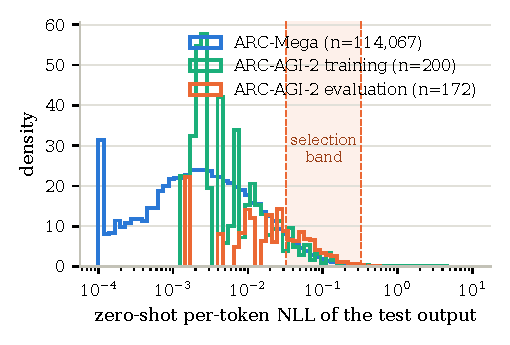
\includegraphics[width=\linewidth]{nll_dist.pdf}
\caption{Per-token NLL under the frozen \nvarc{} model (log-$x$). Shaded: the selection band, the evaluation set's P25--P95.}
\label{fig:nll}
\end{subfigure}\hfill
\begin{subfigure}[t]{0.50\textwidth}
\centering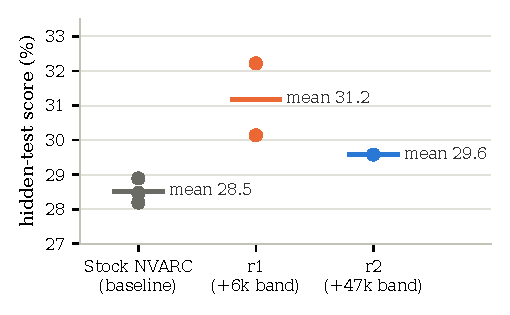
\includegraphics[width=\linewidth]{lb_draws.pdf}
\caption{Hidden-test scores on the ARC Prize 2026 public leaderboard ($\approx$120 hidden tasks). Each dot is one full 12-hour scoring run.}
\label{fig:draws}
\end{subfigure}
\caption{Where the solver finds \mega{} hard (left) and what training on the hard band did (right).}
\end{figure}

\begin{figure}[t]
\centering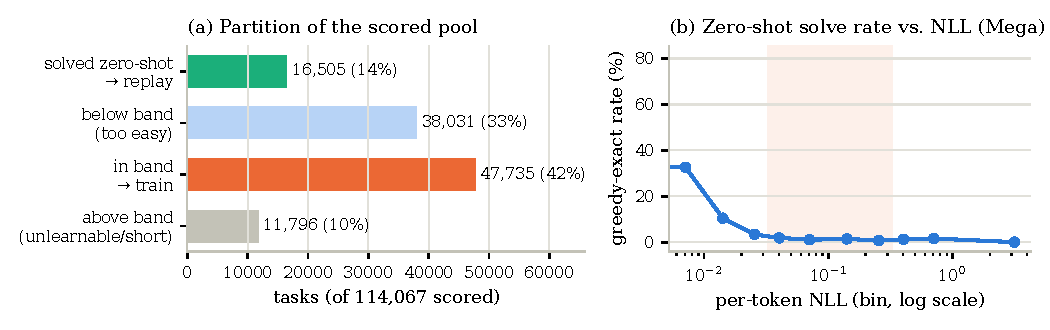
\includegraphics[width=\textwidth]{partition.pdf}
\caption{(a) The band rule partitions the 114{,}067 scored tasks. (b) Greedy-exact rate by NLL bin on \mega{}: the band (shaded) sits where almost nothing is solved zero-shot yet token accuracy is still high (92--99\%).}
\label{fig:partition}
\end{figure}

% =====================================================================
\section{Experiments on the hidden test set}
\label{sec:results}

\paragraph{Setup.}
All scores are ARC Prize 2026 public-leaderboard scores: pass@2 exact match on $\approx$120 hidden tasks, computed by a 12-hour re-run of the submitted notebook on 4$\times$L4 with no internet. Because Kaggle allows one submission per day and the pipeline is stochastic (batched DFS decoding is not batch-invariant~\citep{nvarc2025}), each configuration was scored as many times as the budget allowed. The three stock-checkpoint draws, made with successive versions of the same deadline scaffold (v6--v8), spread by 0.7 points; we treat $\pm1.5$ as the working noise level. Local evaluation accuracy is not reported because the base checkpoint was trained on the public evaluation set (\S\ref{sec:method}); the hidden draws are the only clean signal we have.

\paragraph{Runs.}
Table~\ref{tab:runs} lists the two continuation runs. \textbf{r1} trains on 6{,}000 selected tasks from the first probe batch (plus replay) for one epoch, $\approx$270 optimizer steps, 2.05\,h on one H200. \textbf{r2} trains on all 47{,}435 selected tasks outside the validation split, 2{,}118 steps, 11.7\,h on one RTX PRO 6000 (96\,GB), same hyper-parameters. Both are merged and dropped into the unchanged \nvarc{} notebook.

\begin{table}[t]
\centering\footnotesize\setlength{\tabcolsep}{4pt}
\caption{Continuation runs and outcomes. Losses are nats per output token, step 0 $\to$ end (r2 also at step 800). Hidden-test scores are public-leaderboard draws of the same notebook; only the checkpoint differs.}
\label{tab:runs}
\begin{tabular}{lrrrlll}
\toprule
Run & Selected & Steps & GPU-h & Held-out loss (Mega val.) & Forgetting monitor (eval) & Hidden-test draws (mean) \\
\midrule
baseline & --- & --- & --- & 0.0734 & 0.0724 & 28.89, 28.47, 28.19 (28.5)\\
r1 & 6{,}000 & $\approx$270 & 2.05 & 0.0734 $\to$ 0.0603 ($-18\%$) & 0.0724 $\to$ 0.0692 & \textbf{32.22, 30.14 (31.2)}\\
r2 & 47{,}435 & 2{,}118 & 11.7 & 0.0734 $\to$ 0.0450 ($-39\%$) & 0.0724 $\to$ 0.0707 $\to$ 0.0716 & 29.58 (29.6)\\
\bottomrule
\end{tabular}
\end{table}

\paragraph{Result 1: a small selected set helps.}
r1 scored 32.22 and 30.14 on two independent scoring runs against a baseline mean of 28.5 (Figure~\ref{fig:draws}): $+2.7$ points from 6{,}000 tasks, 0.008\% of the pool's ARC tasks and 0.2\% of the samples \nvarc{} was originally trained on, at a cost of two GPU-hours. The lowest r1 draw exceeds the highest baseline draw by 1.25 points. With two and three draws the difference is suggestive rather than statistically settled (Welch $t\approx2.5$ on one effective degree of freedom); we report it as such. The r1 model is the linked submission.

\begin{figure}[t]
\centering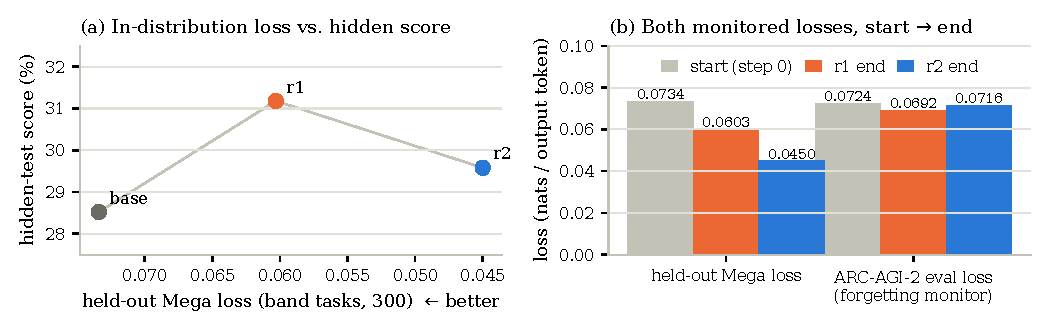
\includegraphics[width=\textwidth]{decoupling.pdf}
\caption{(a) Held-out loss on the selected pool versus hidden-test score: the in-distribution loss keeps improving from r1 to r2 while the hidden score falls back. (b) Both monitored losses at the start and end of each run; only the forgetting monitor orders the runs the way the hidden test does.}
\label{fig:decoupling}
\end{figure}

\paragraph{Result 2: scaling the selected set did not help.}
r2 reached a held-out Mega loss 39\% below the start (Figure~\ref{fig:decoupling})---more than twice r1's improvement on exactly the same 300 validation tasks---yet scored 29.58, below both r1 draws and within noise of the baseline. Had we selected the model by the in-distribution validation loss, as is standard and as \nvarc{}'s authors did with public-evaluation loss, we would have shipped the worse model. The forgetting monitor told a different story: it stood at 0.0707 at step 800 and ended at 0.0716, i.e.\ it rose over the last 1{,}300 steps of r2, while r1 ended at 0.0692.

% =====================================================================
\section{Analysis: why the band works, and why its own loss misleads}
\label{sec:analysis}

\paragraph{What the band selects.}
Figure~\ref{fig:profile} profiles the three NLL regions of the first probe batch against the evaluation set. Tasks below the band are dominated by large outputs that copy most of the input (83\% same-shape, median 504 answer tokens, 99\% token accuracy): the per-token NLL is low because most tokens are trivially predictable, not because the rule is known. Tasks above the band are a distinct population with very short outputs (median 30 tokens, 10\% same-shape): with few copyable tokens every token is a decision and the per-token NLL is high, so the upper cut is largely a \emph{length} filter rather than a difficulty filter. The band itself matches the evaluation set on token accuracy (97\% vs.\ 97\%) and answer length (270 vs.\ 389 tokens) more closely than either tail, which is what anchoring to the benchmark's percentiles is meant to achieve. A length-aware score (e.g.\ NLL restricted to tokens that differ from the input, or a per-task $z$-score) would make the upper cut a genuine difficulty cut; we leave this to future work.

\begin{figure}[t]
\centering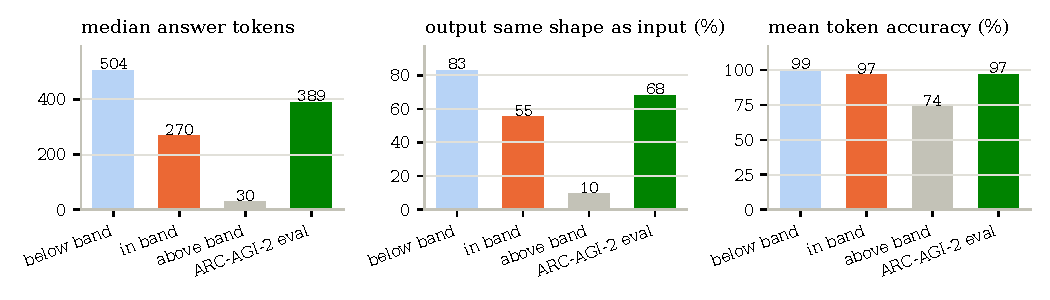
\includegraphics[width=\textwidth]{band_profile.pdf}
\caption{What the band rule selects (first probe batch, 21{,}679 tasks) compared with the public evaluation set. Below-band tasks are long, copy-heavy outputs; above-band tasks are very short outputs; the band resembles the evaluation set.}
\label{fig:profile}
\end{figure}

\paragraph{Why a small selected set helps.}
\nvarc{} adapts to every test task with LoRA TTT, so the base checkpoint's job is not to \emph{know} any particular task but to supply a good prior over rule families and grid regularities from which a few hundred TTT steps can recover the specific rule. The band contains tasks the solver nearly handles (token accuracy 92--99\%) but does not quite (greedy-exact 1--2\%): in the vocabulary of \citet{mindermann2022rholoss}, learnable and not yet learnt. A short continuation on such tasks adjusts the prior where it is weakest, and the forgetting monitor confirms that the base knowledge is not disturbed (0.0724 $\to$ 0.0692).

\paragraph{Why in-distribution held-out loss is the wrong signal.}
The held-out Mega loss measures fit to the \emph{generator distribution} of the selected pool. That distribution differs from ARC-AGI-2 in ways that the band cannot remove: it is produced by a finite family of program generators, 23\% of its rows are augmented copies, and its NLL distribution is wider than the benchmark's. With 8$\times$ more steps at the same learning rate, r2 travels much further from the \nvarc{} optimum and learns Mega-specific regularities that lower Mega loss without improving the prior that TTT needs; the hidden score is flat and the forgetting monitor rises over the last 1{,}300 steps of the run. This is a Goodhart effect specific to solvers with test-time adaptation: the quantity that TTT will fix anyway (task-specific likelihood) is exactly the quantity the validation loss rewards. \nvarc{}'s observation that evaluation-set loss tracked the leaderboard was made during \emph{pre}-training on a broad, benchmark-matched synthetic distribution; our result is that the same proxy fails for \emph{continuation} on a narrower external pool.

\paragraph{The forgetting monitor as an early-stopping signal.}
Across our runs the ordering of final hidden scores (r1 $>$ r2 $\approx$ baseline) is the ordering of final forgetting-monitor values (0.0692 $<$ 0.0716 $<$ 0.0724), and is the \emph{reverse} of the ordering by held-out Mega loss. The monitor costs one evaluation pass over 120 public tasks every 200 steps. We therefore recommend, for any continuation of a TTT-based solver: stop at the first upward turn of the target-benchmark loss, and ignore the in-distribution validation loss for model selection. A noisy-but-clean hidden draw remains the final arbiter.

\paragraph{What a practitioner should take from this.}
(i) Score the pool with the solver before training on it; one forward pass per task is cheap enough to do for $10^5$--$10^6$ tasks on competition hardware. (ii) Train briefly on the band, replay what is already solved. (iii) Watch the target benchmark's loss for a rise, not the pool's loss for a fall. (iv) Expect single-digit-thousand selected tasks to be enough; more is not better without a second lever (lower learning rate, mixed sources, or a length-aware score).

% =====================================================================
\section{Levers we measured and rejected}
\label{sec:negative}
Under the same solo budget we evaluated three other routes to a higher score. Each was measured on the public evaluation set with paired per-task comparisons against the stock \nvarc{} run; we report them so that the completeness criterion is met and so that others can skip them.

\begin{itemize}
\item \textbf{Answer re-ranking.} \nvarc{} generates candidate grids by DFS and ranks them by an augmentation-consistency score. On the 120 public evaluation tasks the stock rule scores 33.3 task-points; a perfect oracle over the same candidates would score 38.5 (54 of 172 outputs have a correct candidate). The best of 14 alternative rules (\texttt{probmul\_3}, which sums candidate and augmentation log-probabilities) recovered only $+0.5$ task-points: in 8 of 9 recoverable misses the wrong answer out-scored the right one on \emph{every} signal. The headroom is real but the model is confidently wrong, so re-ranking cannot reach it.
\item \textbf{CPU program search.} The 2020 winning DSL search~\citep{wind2020icecuber} at depth 3 solved 2.5 task-points on the evaluation set in 55 CPU-minutes, only 0.5 beyond \nvarc{}; worth filling empty attempt slots, not worth displacing a transductive attempt.
\item \textbf{Test-time program induction with open 30B-class models.} We built a multi-round propose--execute--verify loop in the exact tool format of NVIDIA's ARC agentic traces~\citep{nemotronarc2026}, with a verifier that checks demonstration pass, leave-one-out generalisation, literal-grid hygiene and cross-program consensus. On 57 development tasks the best zero-shot model (Qwen3.6-35B-A3B) produced final programs that passed all demonstrations in 2 of 122 cases, truncated 37\% of its reasoning turns, and solved nothing \nvarc{} missed; in a preceding 5-task smoke test two other models (Nemotron-3-Nano-30B, Qwen3-30B-Thinking) truncated 98--100\% of their turns and produced no programs. Without fine-tuning on such traces, induction at this model size is not competitive inside 12 hours on L4s. A reusable finding from this branch: verifiers also have \emph{false negatives}---correct programs were rejected because the model's own test code embedded demonstration grids---fixed by verifying only the code reachable from the solution function.
\end{itemize}

% =====================================================================
\section{Limitations}
Our evidence is six hidden-test draws across three configurations with a noise floor of about $\pm1.5$ points; the $+2.7$ effect is consistent across both r1 draws but is not established beyond doubt. We ran one base model, one seed per configuration and one learning rate, so we cannot separate ``too much data'' from ``too many steps at this learning rate''; a 6k run with random rather than band selection is the control we most wanted and could not afford before the deadline. The upper cut is partly a length filter (\S\ref{sec:analysis}). Public-leaderboard scores use about half of the hidden tasks; private scores may differ. Finally, the target profile used in the probe was chosen by inspection of \nvarc{} misses and is a confound: the band was tested only on profile-matched tasks.

% =====================================================================
\section{Conclusion}
A strong ARC solver can tell you which synthetic tasks are worth its training time: score the pool once with the solver's own likelihood, keep what lies in the benchmark's difficulty band and is not yet solved, replay what is. Six thousand such tasks and two GPU-hours moved the 2025 winner by $+2.7$ points on the 2026 hidden test set; forty-seven thousand did not move it further, even as the in-distribution loss fell by 39\%. The method requires nothing but a likelihood-assigning solver and a target benchmark, so it transfers directly to any few-shot induction setting with a synthetic pool; the lesson about validation signals transfers to any solver that adapts at test time.

\paragraph{Reproducibility.}
Code (probe, scoring notebook, data builder, training kit, selection lab) and the linked Kaggle notebook and model are listed in Appendix~\ref{app:repro}.

\paragraph{Acknowledgements.}
We thank the \nvarc{} authors for releasing their code and checkpoint, and MindsAI/Tufa Labs for releasing \mega{}.

\bibliographystyle{plainnat}
\bibliography{refs}

\clearpage
\appendix
\section{Reproducibility details}
\label{app:repro}

\paragraph{Linked submission.}
Kaggle notebook \emph{NVARC updated}, version 9 (``v9 mega-r1 smoke), \url{https://www.kaggle.com/code/harthikrm/nvarc-updated?scriptVersionId=356815178}; model \texttt{harthikrm/nvarc-mega-r1} (v1); public-leaderboard score 32.22 (second draw of the same version: 30.14). Code: \url{https://github.com/harthikrm/arc-prize-2026-paper}.

\paragraph{Competition-time pipeline.}
The public \nvarc{} notebook (pinned Kaggle environment of 2025-07-07, Unsloth with the flash-attention patch) with three changes: a glob that resolves the model directory (\texttt{NVARC\_MODEL\_DIR}); a placeholder \texttt{submission.json} written in the first minute covering all hidden task IDs; and a \texttt{StopAtDeadline} callback that halts test-time training at 11.75\,h so the 12-hour limit cannot zero the run. Per-task TTT (LoRA $r{=}256$, $\alpha{=}32$, bf16), batched DFS decoding with a per-task cap, and the stock augmentation re-scoring rule are unchanged.

\paragraph{Scoring notebook.}
Four worker processes (one per L4), teacher-forced forward passes over length-sorted batches with a 24{,}576-token budget, right padding, bf16, SDPA attention; outputs \texttt{mega\_scores.csv} with per-output \texttt{nll\_mean}, \texttt{nll\_sum}, \texttt{greedy\_exact}, \texttt{frac\_tokens\_correct} and \texttt{n\_train\_used}. Throughput 13.6k tasks/h.

\paragraph{Probe.}
\begin{quote}\small\ttfamily mega\_probe.py --max-gb 15 --max-tasks-per-file 20000 --exclude <earlier batch>\end{quote}
Dedup hash: minimum over D8 of a blake2b digest of the colour-rank-relabelled grid; evaluation firewall: any demonstration grid or test input with more than nine cells that matches a public-evaluation grid under D8 rejects the task; dedup uses the first demonstration input; target profile: $\ge$5 colours, $\ge$300 cells, $\ge$3 four-connected non-background components in the first demonstration input.

\paragraph{Data builder.}
\begin{quote}\small\ttfamily build\_train\_data.py --mega mega\_sample [--mega mega\_big]\\ \phantom{xx}--eval-quantile 0.25 --eval-upper-quantile 0.95 --max-train 6000|60000\\ \phantom{xx}--n-val 300 --reuse-val train\_data/val.json\end{quote}
Thresholds computed from the 172 evaluation outputs: $\tau_{25}=0.03236$, $\tau_{95}=0.32646$. Replay = greedy-solved Mega tasks + 1{,}000 public training tasks.

\paragraph{Training.}
\begin{quote}\small\ttfamily train\_lora.py --rank 128 --alpha 32 --lr 5e-5 --warmup 0.03 --global-batch 32\\ \phantom{xx}--max-len 8192 --n-aug 1 --replay-frac 0.3 --eval-steps 200\\ \phantom{xx}--arc-eval <public eval>\end{quote}
rsLoRA on \texttt{q,k,v,o,gate,up,down}; cosine schedule; max grad-norm 1.0; no weight decay; seed 42; \texttt{eval\_on\_start}; timed full-state checkpoints pushed to a private Hugging Face repo for provider hopping. r1: one H200 (Lightning AI), gradient checkpointing on, 2.05\,h. r2: one RTX PRO 6000 96\,GB (Colab), gradient checkpointing off, 11.7\,h, 2{,}118 steps; intermediate forgetting-monitor value 0.0707 at step 800. Merge: \texttt{--merge} writes the merged bf16 model with \nvarc{}'s extra loader files, uploaded via \texttt{kagglehub}.

\paragraph{Grid statistics used in \S\ref{sec:mega}--\S\ref{sec:analysis}.}
Computed on the first demonstration input/output of each task: public evaluation (120 tasks) mean 5.37 colours, 351 cells, 68\% same-shape; public training (1{,}000 tasks) mean 3.84 colours, 161 cells, 67\% same-shape; selected \mega{} tasks (first batch) mean 6.6 colours, 501 cells, 55\% same-shape.

\paragraph{Noise.}
Three stock-checkpoint draws under successive scaffold versions scored 28.89, 28.47 and 28.19 (SD 0.35); the two r1 draws differ by 2.08. An unmodified copy of the original public \nvarc{} notebook, without the deadline scaffold, scored 31.53 in one draw at the start of the competition; all comparisons in this paper are between notebooks that share the scaffold.

\end{document}
